% ============================================================
% LIBRARY MONITORING SYSTEM — MPMC PROJECT REPORT
% NMIMS STME, Chandigarh
% ============================================================

\documentclass[12pt,a4paper]{article}

% ─── Packages ────────────────────────────────────────────────
\usepackage[a4paper, margin=2.5cm]{geometry}
\usepackage{graphicx}
\usepackage{float}
\usepackage{amsmath}
\usepackage{amssymb}
\usepackage{xcolor}
\usepackage{hyperref}
\usepackage{listings}
\usepackage{booktabs}
\usepackage{array}
\usepackage{tabularx}
\usepackage{multirow}
\usepackage{enumitem}
\usepackage{fancyhdr}
\usepackage{titlesec}
\usepackage{tocloft}
\usepackage{setspace}
\usepackage{caption}
\usepackage{subcaption}
\usepackage{mdframed}
\usepackage{tikz}
\usetikzlibrary{shapes.geometric, arrows.meta, positioning, calc}

% ─── Colors ──────────────────────────────────────────────────
\definecolor{primary}{RGB}{25, 70, 140}
\definecolor{accent}{RGB}{0, 120, 180}
\definecolor{codebg}{RGB}{245, 247, 250}
\definecolor{codeframe}{RGB}{200, 210, 225}
\definecolor{good}{RGB}{0, 150, 100}
\definecolor{warn}{RGB}{180, 130, 0}
\definecolor{danger}{RGB}{180, 50, 50}

% ─── Hyperref ────────────────────────────────────────────────
\hypersetup{
  colorlinks  = true,
  linkcolor   = primary,
  urlcolor    = accent,
  citecolor   = primary,
  pdftitle    = {Library Monitoring System — MPMC Project Report},
  pdfauthor   = {NMIMS STME},
}

% ─── Section Styling ─────────────────────────────────────────
\titleformat{\section}{\large\bfseries\color{primary}}{}{0em}{}[\titlerule]
\titleformat{\subsection}{\normalsize\bfseries\color{accent}}{}{0em}{}
\titleformat{\subsubsection}{\normalsize\itshape}{}{0em}{}

% ─── Header / Footer ─────────────────────────────────────────
\pagestyle{fancy}
\fancyhf{}
\fancyhead[L]{\small\color{primary}Library Monitoring System}
\fancyhead[R]{\small\color{primary}NMIMS STME — MPMC Project}
\fancyfoot[C]{\small\thepage}
\renewcommand{\headrulewidth}{0.4pt}

% ─── Code Listings ───────────────────────────────────────────
\lstdefinestyle{cppstyle}{
  language        = C++,
  backgroundcolor = \color{codebg},
  frame           = single,
  framesep        = 4pt,
  rulecolor       = \color{codeframe},
  basicstyle      = \ttfamily\footnotesize,
  keywordstyle    = \bfseries\color{primary},
  commentstyle    = \itshape\color{gray},
  stringstyle     = \color{good},
  numberstyle     = \tiny\color{gray},
  numbers         = left,
  numbersep       = 8pt,
  breaklines      = true,
  captionpos      = b,
  tabsize         = 2,
  showstringspaces= false,
}

\lstset{style=cppstyle}

% ─── Table Styling ───────────────────────────────────────────
\renewcommand{\arraystretch}{1.4}

% ─── Double Spacing for report ───────────────────────────────
\onehalfspacing

% ============================================================
\begin{document}

% ─── Cover Page ──────────────────────────────────────────────
\begin{titlepage}
\centering
\vspace*{1cm}

{\color{primary}\rule{\linewidth}{0.8pt}}
\vspace{0.4cm}

{\fontsize{26}{32}\selectfont\bfseries\color{primary}
Library Monitoring System}

\vspace{0.2cm}
{\Large\color{accent} Smart IoT-Based Environment \& Occupancy Monitor}

\vspace{0.4cm}
{\color{primary}\rule{\linewidth}{0.8pt}}

\vspace{2cm}

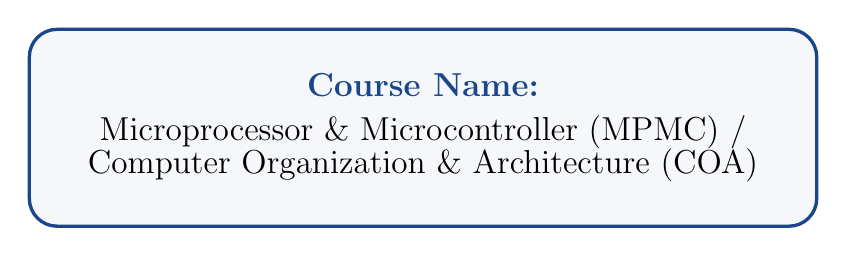
\begin{tikzpicture}
  \node[draw=primary, rounded corners=10pt, fill=codebg, 
        minimum width=10cm, minimum height=2.5cm, align=center,
        line width=1.2pt] {
    {\large\bfseries\color{primary}Course Name:}\\[4pt]
    {\large Microprocessor \& Microcontroller (MPMC) /}\\
    {\large Computer Organization \& Architecture (COA)}
  };
\end{tikzpicture}

\vspace{1.5cm}

\begin{tabular}{rl}
  \textbf{\color{primary}Project Title:}   & Library Monitoring System \\[6pt]
  \textbf{\color{primary}Submitted By:}    & Priyansh Saxena \\[4pt]
                                            & Bria Jain \ | \ Ridhima Rathi \\[6pt]
  \textbf{\color{primary}Section/Semester:}& Section 2 — Semester 4 \\[6pt]
  \textbf{\color{primary}Department:}      & School of Technology Management \& Engineering \\[6pt]
  \textbf{\color{primary}University:}      & SVKM's NMIMS, Indore \\[6pt]
  \textbf{\color{primary}Application Link:}& \url{https://library-monitor-65ad9.web.app} \\[6pt]
  \textbf{\color{primary}Submission Date:} & \today \\
\end{tabular}

\vfill


\begin{tikzpicture}
  \draw[primary, line width=1pt] (0,0) -- (\linewidth,0);
\end{tikzpicture}

{\small\color{gray} Hardware-Only Project · ESP32 · IoT · Firebase Cloud}\\[4pt]
{\tiny\color{gray} Wiring Diagram: \texttt{wiring\_diagram.html}}

\end{titlepage}

\newpage

% ─── Abstract ────────────────────────────────────────────────
\section*{Abstract}
\addcontentsline{toc}{section}{Abstract}

Libraries are passive environments — administrators have no real-time visibility into whether the space is comfortable, crowded, or conducive to study. This project presents the \textbf{Library Monitoring System}, an IoT-based solution built on the ESP32 microcontroller that continuously monitors six physical parameters: temperature, humidity, noise level, air quality, human occupancy, and motion activity.

The system employs two HC-SR04 ultrasonic sensors in a directional configuration to count people entering and exiting, a DHT22 for temperature and humidity, a microphone module for ambient sound level, and an MQ-2 gas sensor as an air quality proxy. An on-board Comfort Index (0–100) is computed from all parameters and pushed to the \textbf{Firebase Realtime Database} every five seconds. A visually polished \textbf{Mobile Web App (PWA)} renders live metrics, trend graphs, and provides remote control features for parameters like capacity limits and buzzer alerts.

Key outcomes include: (1) a functional people-counter accurate within one individual per crossing, (2) real-time cloud logging accessible on any device, (3) LED and buzzer actuators that respond to threshold breaches, and (4) a mobile interface built with the Firebase Web SDK that allows library administrators to remotely set capacity limits and toggle alerts. The system demonstrates microcontroller-based signal acquisition, interrupt-free sensor polling, Firebase bidirectional streaming, and modern PWA architecture.

\vspace{0.3cm}
\noindent\textbf{Keywords:} ESP32, IoT, Firebase, DHT22, HC-SR04, MQ-2, PWA, Occupancy Counting, Environment Monitoring

\newpage

% ─── Table of Contents ───────────────────────────────────────
\tableofcontents
\newpage

% ============================================================
\section{Introduction}

\subsection{Background of the Topic}

The modern library faces a challenge that infrastructure alone cannot solve: the gap between physical environment quality and student awareness. A student leaving a hostel room to find a study space has no way of knowing whether the library is comfortable, crowded, or noisy — until they are already there.

Simultaneously, library administrators lack instrumented data on their space. Without sensors, decisions about air conditioning capacity, seating arrangements, and operating hours are made on anecdote rather than evidence.

The convergence of low-cost microcontrollers, MEMS sensors, and cloud IoT platforms makes it possible to close this gap entirely — at a cost comparable to a single textbook.

\subsection{Importance of Microprocessors and Microcontrollers}

The ESP32, a 32-bit dual-core Xtensa LX6 microcontroller operating at up to 240 MHz, exemplifies the democratization of embedded computing. Unlike its predecessors (the 8-bit Arduino family), the ESP32 integrates:

\begin{itemize}[leftmargin=1.5cm]
  \item Dual-core processing for concurrent sensor polling and WiFi handling
  \item Built-in 802.11 b/g/n WiFi and Bluetooth 4.2
  \item 18 ADC channels (12-bit resolution) for analog sensor interfacing
  \item Hardware UART, SPI, I2C, and PWM peripherals
  \item Deep sleep modes drawing as low as 10 µA for battery applications
\end{itemize}

This project leverages the ESP32's ADC for analog sensor reading, GPIO for digital sensors and actuators, and its WiFi stack for cloud connectivity — making it ideal for a complete IoT pipeline on a single chip.

\subsection{Objective of the Project}

\begin{enumerate}[leftmargin=1.5cm]
  \item Measure \textbf{five or more physical parameters} using appropriate sensors
  \item Implement \textbf{directional occupancy counting} using dual ultrasonic sensors
  \item Drive \textbf{three actuators} (LED green, LED red, buzzer) based on sensor thresholds
  \item Transmit all data to \textbf{Firebase Realtime Database} for remote monitoring
  \item Build a \textbf{custom Mobile Web App (PWA)} for visual analytics
  \item Allow remote \textbf{actuator control} via the custom mobile interface
\end{enumerate}

\newpage

% ============================================================
\section{Problem Statement}

\begin{mdframed}[linecolor=primary, linewidth=1.2pt, leftmargin=0.5cm, rightmargin=0.5cm]
\textit{"Design and implement a smart library monitoring system using the ESP32 microcontroller that measures environmental parameters in real time, tracks occupancy through directional people-counting, logs all data to the cloud, and provides both physical and remote alerts when conditions fall below acceptable thresholds."}
\end{mdframed}

\vspace{0.5cm}

\noindent Concretely, the system must answer four questions that currently go unanswered in a typical library:

\begin{center}
\begin{tabular}{c p{5cm} p{7cm}}
\toprule
\textbf{\#} & \textbf{Question} & \textbf{How the System Answers} \\
\midrule
1 & Is it worth going right now? & Comfort Score broadcast via Firebase/App \\
2 & Is the air quality acceptable? & MQ-2 sensor with threshold alert \\
3 & How crowded is it? & Dual HC-SR04 directional counter \\
4 & Is it quiet enough to study? & Microphone module with dB proxy \\
\bottomrule
\end{tabular}
\end{center}

\newpage

% ============================================================
\section{System Design}

\subsection{Block Diagram}

\begin{figure}[H]
\centering
\begin{tikzpicture}[
  node distance = 1.5cm and 2cm,
  box/.style    = {rectangle, draw=primary, rounded corners=5pt, 
                   fill=codebg, minimum width=2.8cm, minimum height=0.9cm,
                   align=center, font=\small},
  cloud/.style  = {ellipse, draw=accent, fill=blue!5, 
                   minimum width=3cm, minimum height=1cm, align=center, font=\small},
  arr/.style    = {-{Latex[length=3mm]}, thick, color=primary},
]

% Sensors column
\node[box] (dht)  {DHT22\\Temp/Humid};
\node[box, below=0.5cm of dht]  (pir)  {PIR Sensor\\Motion};
\node[box, below=0.5cm of pir]  (mic)  {Mic Module\\Noise};
\node[box, below=0.5cm of mic]  (gas)  {MQ-2 Gas\\Air Quality};
\node[box, below=0.5cm of gas]  (us1)  {HC-SR04 \#1\\Entry};
\node[box, below=0.5cm of us1]  (us2)  {HC-SR04 \#2\\Exit};

% ESP32
\node[box, right=3cm of pir, minimum width=3cm, minimum height=7cm,
      fill=blue!8, draw=primary, line width=1.5pt, font=\normalsize\bfseries,
      label={[font=\footnotesize, color=gray]below:240 MHz · Dual Core}]
      (esp) {ESP32\\DevKit v1\\\\ADC · GPIO\\WiFi Stack\\Timer ISR};

\node[box, right=3cm of esp, yshift=2cm] (ledr) {LED Red\\Overload Alert};
\node[box, below=0.35cm of ledr] (ledg) {LED Green\\Status OK};
\node[box, below=0.35cm of ledg] (buzz) {Buzzer\\Audio Alert};
\node[box, below=0.35cm of buzz] (lcd) {I2C LCD 16x2\\Local Feedback};

% Cloud
\node[cloud, above=2cm of esp] (firebase) {Firebase\\Cloud};
\node[cloud, right=1.5cm of blynk]  (dash)  {Mobile Web\\App (PWA)};

% Arrows: sensors → ESP32
\draw[arr] (dht) -- (esp);
\draw[arr] (pir) -- (esp);
\draw[arr] (mic) -- (esp);
\draw[arr] (gas) -- (esp);
\draw[arr] (us1) -- (esp);
\draw[arr] (us2) -- (esp);

% Arrows: ESP32 → actuators
\draw[arr] (esp) -- (ledr);
\draw[arr] (esp) -- (ledg);
\draw[arr] (esp) -- (buzz);
\draw[arr] (esp) -- (lcd);

% Arrows: ESP32 ↔ Cloud
\draw[arr, <->, color=accent] (esp) -- node[left, font=\tiny]{WiFi} (firebase);
\draw[arr, color=accent] (firebase) -- node[above, font=\tiny]{WebSocket} (dash);

\end{tikzpicture}
\caption{System Block Diagram — Library Monitoring System}
\end{figure}

\subsection{Functional Description}

The system operates on a continuous polling loop with a 2-second sampling interval. On each cycle:

\begin{enumerate}[leftmargin=1.5cm]
  \item DHT22 is queried over single-wire protocol; temperature and humidity are stored
  \item PIR digital output is read; a \texttt{HIGH} signal indicates motion presence
  \item Microphone and gas sensor analog outputs are read via the ESP32 12-bit ADC (GPIO 34, 35)
  \item Both HC-SR04 sensors are triggered sequentially; duration is measured with \texttt{pulseIn()}
  \item Distance is computed using temperature-corrected speed of sound: $v = 331.3 + 0.606 \times T$
  \item Occupancy logic determines entry/exit based on which sensor triggers first
  \item Comfort Score is computed from all parameters
  \item All values are pushed to Firebase Realtime Database every 5 seconds
  \item ESP32 listens to a Firebase Stream for remote capacity/buzzer updates
  \item LEDs and buzzer are updated based on local thresholds and remote commands
\end{enumerate}

\newpage

\subsection{Hardware Requirements}

\begin{table}[H]
\centering
\caption{Bill of Materials}
\begin{tabularx}{\textwidth}{c X c c c}
\toprule
\textbf{\#} & \textbf{Component} & \textbf{Qty} & \textbf{Interface} & \textbf{Est. Cost (₹)} \\
\midrule
1  & ESP32 DevKit v1 (38-pin)         & 1 & —         & 400 \\
2  & DHT22 Temperature/Humidity Sensor & 1 & 1-Wire    & 120 \\
3  & HC-SR04 Ultrasonic Sensor         & 2 & GPIO      & 120 \\
4  & PIR HC-SR501 Motion Sensor        & 1 & GPIO      & 60  \\
5  & Microphone Sound Module (KY-037)  & 1 & Analog    & 50  \\
6  & MQ-2 Gas/Smoke Sensor             & 1 & Analog    & 80  \\
7  & LED (Red)                         & 1 & GPIO      & 5   \\
8  & LED (Green)                       & 1 & GPIO      & 5   \\
9  & Passive Buzzer                    & 1 & GPIO      & 10  \\
10 & I2C LCD 16x2 Display              & 1 & I2C       & 180 \\
11 & Breadboard (830 tie-point)        & 1 & —         & 50  \\
12 & Resistors (220Ω, 1kΩ, 4.7kΩ)     & Asst. & —    & 20  \\
13 & Jumper Wires                      & Asst. & —     & 30  \\
\midrule
   & \textbf{Total}                    & & & \textbf{≈ ₹1130} \\
\bottomrule
\end{tabularx}
\end{table}

\subsection{Software Requirements}

\begin{itemize}[leftmargin=1.5cm]
  \item \textbf{IDE:} Arduino IDE 2.x with ESP32 board support (Espressif Systems, v2.0+)
  \item \textbf{Language:} C++ (Arduino framework)
  \item \textbf{Libraries:}
    \begin{itemize}
      \item \texttt{DHT.h} — Adafruit DHT sensor library
      \item \texttt{Firebase\_ESP\_Client.h} — Firebase Realtime Database library
      \item \texttt{WiFi.h} — ESP32 WiFi stack (built-in)
    \end{itemize}
  \item \textbf{Cloud:} Firebase Realtime Database (Google Cloud)
  \item \textbf{Mobile App:} PWA (HTML5 / CSS3 / Firebase Web SDK v10)
\end{itemize}

\newpage

% ============================================================
\section{Circuit Diagram}

\subsection{Pin Assignment Table}

\begin{table}[H]
\centering
\caption{ESP32 GPIO Pin Assignments}
\begin{tabular}{l l l p{5cm}}
\toprule
\textbf{Component} & \textbf{Pin/Signal} & \textbf{ESP32 GPIO} & \textbf{Notes} \\
\midrule
DHT22             & DATA   & GPIO 4  & 4.7kΩ pull-up to 3.3V required \\
LCD 16x2 SDA      & DATA   & GPIO 21 & Standard I2C Data pin \\
LCD 16x2 SCL      & CLOCK  & GPIO 22 & Standard I2C Clock pin \\
PIR HC-SR501      & OUT    & GPIO 14 & Adjust onboard sensitivity trimmer \\
Mic Module        & AO     & GPIO 34 & Input-only ADC pin \\
MQ-2 Gas Sensor   & AO     & GPIO 35 & Input-only ADC pin; 24h preheat \\
HC-SR04 \#1 (Entry) & TRIG & GPIO 26 & 10µs pulse to trigger \\
HC-SR04 \#1 (Entry) & ECHO & GPIO 27 & 5V output → use voltage divider \\
HC-SR04 \#2 (Exit)  & TRIG & GPIO 32 & 10µs pulse to trigger \\
HC-SR04 \#2 (Exit)  & ECHO & GPIO 33 & 5V output → use voltage divider \\
LED Green         & Anode  & GPIO 18 & 220Ω series resistor \\
LED Red           & Anode  & GPIO 19 & 220Ω series resistor \\
Buzzer            & +      & GPIO 23 & NPN transistor driver recommended \\
\bottomrule
\end{tabular}
\end{table}

\subsection{Important Wiring Notes}

\begin{enumerate}[leftmargin=1.5cm]
  \item \textbf{HC-SR04 ECHO pin voltage divider:} The HC-SR04 operates at 5V; its ECHO output is 5V logic. The ESP32 GPIO tolerates a maximum of 3.3V. Use a voltage divider: $R_1 = 1k\Omega$ (ECHO to ESP), $R_2 = 2k\Omega$ (ESP to GND). This gives $V_{out} = 5 \times \frac{2000}{3000} = 3.33V \approx 3.3V$.
  
  \item \textbf{MQ-2 power:} Requires 5V supply and significant warm-up current (approximately 150mA peak). Power from the USB 5V rail via breadboard, not from the ESP32's 3.3V regulator.
  
  \item \textbf{DHT22 pull-up:} The single-wire data line requires a 4.7kΩ pull-up resistor to 3.3V for reliable communication.
  
  \item \textbf{Common GND:} All GNDs (ESP32, sensors, actuators) must share a common ground rail on the breadboard.
\end{enumerate}

\newpage

% ============================================================
\section{Algorithm and Flowchart}

\subsection{Main Algorithm}

\begin{mdframed}[linecolor=accent, leftmargin=0.3cm, rightmargin=0.3cm]
\textbf{Pseudocode — Main Loop (2s interval)}
\begin{enumerate}[leftmargin=1cm, label=\textbf{Step \arabic*:}]
  \item Read DHT22 → store \texttt{temperature}, \texttt{humidity}
  \item Read PIR digital → store \texttt{pirState}
  \item Read MIC analog (ADC) → store \texttt{noiseLevel}
  \item Read GAS analog (ADC) → store \texttt{airQuality}
  \item Trigger US1; measure \texttt{d1} = $\frac{duration \times v_{sound}}{2}$
  \item Trigger US2; measure \texttt{d2}
  \item \textbf{Occupancy logic:}
    \begin{itemize}
      \item If US1 triggers before US2 → \texttt{count++} (entry)
      \item If US2 triggers before US1 → \texttt{count--} (exit)
      \item Debounce: minimum 1000ms between events
    \end{itemize}
  \item Compute ComfortScore = $f(\text{temp, humid, noise, air, occupancy})$
  \item Update LEDs and buzzer
  \item (Every 5s) Push all values to Firebase nodes at \texttt{/sensor}
  \item Listen to \texttt{/controls} stream for remote updates
\end{enumerate}
\end{mdframed}

\vspace{0.5cm}

\subsection{Comfort Score Formula}

The Comfort Score $C$ is defined as:

\begin{equation}
C = \max\left(0, \ 100 - P_T - P_H - P_N - P_A - P_O\right)
\end{equation}

Where:
\begin{align*}
P_T &= 3 \times \max(0, T - 30)          && \text{Temperature penalty (per °C above 30°C)} \\
P_H &= 2 \times \max(0, H - 70)          && \text{Humidity penalty (per \% above 70\%)} \\
P_N &= 20 \times \mathbb{1}[\text{ADC\_noise} > 2500] && \text{Noise threshold penalty} \\
P_A &= 25 \times \mathbb{1}[\text{ADC\_gas}   > 2000] && \text{Air quality penalty} \\
P_O &= 30 \times \mathbb{1}[\text{count} \geq \text{maxCap}] && \text{Overcrowding penalty}
\end{align*}

\subsection{Flowchart}

\begin{figure}[H]
\centering
\begin{tikzpicture}[
  node distance=0.8cm,
  startstop/.style={rounded rectangle, draw=primary, fill=blue!10, minimum width=3cm, minimum height=0.7cm, font=\small},
  process/.style  ={rectangle,         draw=primary, fill=codebg,  minimum width=4cm, minimum height=0.7cm, font=\small},
  decision/.style ={diamond, aspect=2, draw=accent,  fill=yellow!8,minimum width=4cm, font=\scriptsize},
  arr/.style={-{Latex[length=2.5mm]}, thick, primary},
]
\node[startstop] (start) {START};
\node[process, below=of start] (init) {Initialize pins, DHT22, WiFi, Firebase};
\node[process, below=of init]  (read) {Read all sensors (2s timer)};
\node[process, below=of read]  (occ)  {Handle occupancy (dual US)};
\node[process, below=of occ]   (comp) {Compute Comfort Score};
\node[decision, below=of comp] (thr)  {Any threshold breached?};
\node[process, right=2cm of thr] (act) {Trigger LED Red + Buzzer};
\node[process, below=of thr]   (grn)  {LED Green ON};
\node[process, below=of grn]   (blnk) {Push to Firebase (5s timer)};
\node[process, below=of blnk]  (wait) {Wait for next timer tick};

\draw[arr] (start)--(init);
\draw[arr] (init) --(read);
\draw[arr] (read) --(occ);
\draw[arr] (occ)  --(comp);
\draw[arr] (comp) --(thr);
\draw[arr] (thr)  --node[above, font=\tiny]{YES} (act);
\draw[arr] (thr)  --node[left,  font=\tiny]{NO}  (grn);
\draw[arr] (act)  |- (blnk);
\draw[arr] (grn)  --(blnk);
\draw[arr] (blnk) --(wait);
\draw[arr] (wait.east) -- ++(1.5,0) |- (read.east);
\end{tikzpicture}
\caption{Main Program Flowchart}
\end{figure}

\newpage

% ============================================================
\section{Program Code}

\subsection{Core Sensor Reading and Distance Calculation}

\begin{lstlisting}[caption={Temperature-Compensated Distance Measurement}]
float readDistance(int trigPin, int echoPin) {
  // Use DHT22 temperature for accurate speed of sound
  float speedOfSound = 331.3 + (0.606 * temperature);

  digitalWrite(trigPin, LOW);
  delayMicroseconds(2);
  digitalWrite(trigPin, HIGH);
  delayMicroseconds(10);
  digitalWrite(trigPin, LOW);

  long duration = pulseIn(echoPin, HIGH, 30000); // 30ms timeout
  if (duration == 0) return 999.0; // No echo received
  return (duration * speedOfSound / 10000.0) / 2.0; // cm
}
\end{lstlisting}

\subsection{Occupancy Counting Logic}

\begin{lstlisting}[caption={Directional People Counter Using Dual Ultrasonics}]
void handleOccupancy() {
  float d1 = readDistance(TRIG1_PIN, ECHO1_PIN); // Entry side
  float d2 = readDistance(TRIG2_PIN, ECHO2_PIN); // Exit side
  unsigned long now = millis();

  // Entry: US1 triggers first, then US2 within 3 seconds
  if (d1 < DISTANCE_TRIGGER_CM && !entry1Triggered) {
    entry1Triggered = true;
    lastEntry1 = now;
  }
  if (entry1Triggered && d2 < DISTANCE_TRIGGER_CM) {
    if ((now - lastEntry1) < 3000) {
      occupancyCount++;
    }
    entry1Triggered = false;
  }

  // Exit: US2 triggers first, then US1 within 3 seconds  
  if (d2 < DISTANCE_TRIGGER_CM && !entry2Triggered) {
    entry2Triggered = true;
    lastEntry2 = now;
  }
  if (entry2Triggered && d1 < DISTANCE_TRIGGER_CM) {
    if ((now - lastEntry2) < 3000 && occupancyCount > 0) {
      occupancyCount--;
    }
    entry2Triggered = false;
  }
}
\end{lstlisting}

\subsection{Comfort Score Computation}

\begin{lstlisting}[caption={Composite Comfort Score (0--100)}]
int computeComfortScore() {
  int score = 100;

  if (temperature > TEMP_MAX)
    score -= (int)((temperature - TEMP_MAX) * 3);
  if (humidity > HUMIDITY_MAX)
    score -= (int)((humidity - HUMIDITY_MAX) * 2);
  if (noiseLevel > NOISE_THRESHOLD) score -= 20;
  if (airQuality  > GAS_THRESHOLD)  score -= 25;
  if (occupancyCount >= maxCapacity) score -= 30;

  return constrain(score, 0, 100);
}
\end{lstlisting}

\newpage

% ============================================================
\section{Working and Implementation}

\subsection{Input → Process → Output Flow}

\begin{center}
\begin{tabular}{p{4cm} p{5.5cm} p{4.5cm}}
\toprule
\textbf{Input (Sensors)} & \textbf{Process (ESP32)} & \textbf{Output (Actuators + Cloud)} \\
\midrule
DHT22: T = 28°C, H = 55\% & Normal range; no penalty & LED Green ON \\
MQ-2: ADC = 2500 (high) & $P_A = 25$; score drops & Buzzer alert + Mobile Notification \\
HC-SR04: d1 < 80cm then d2 & Entry event detected & count++ \\
HC-SR04: d2 < 80cm then d1 & Exit event detected & count-- \\
PIR: HIGH + count $\geq$ maxCap & Overcrowding confirmed & LED Red, Buzzer, Firebase push \\
Mic: ADC = 3100 & Noise threshold breached & Mobile App alert \\
\bottomrule
\end{tabular}
\end{center}

\subsection{Role of Timers}

The ESP32 uses non-blocking timers to schedule sensor samples and cloud sync. Three main cycles are defined:

\begin{itemize}[leftmargin=1.5cm]
  \item \textbf{2000ms cycle:} \texttt{readAllSensors()} — reads all six sensors
  \item \textbf{2000ms cycle:} \texttt{handleOccupancy()} — processes ultrasonic pair
  \item \textbf{5000ms cycle:} \texttt{pushToFirebase()} — serializes data to JSON and syncs
\end{itemize}

This architecture avoids \texttt{delay()} calls entirely, keeping the main loop responsive to Firebase stream callbacks and ensuring consistent sampling intervals.

\subsection{Temperature Correction for Ultrasonic}

Standard tutorials use a fixed speed of sound (343 m/s). This system improves accuracy by computing the actual speed from the DHT22 reading:

\[
v_{\text{sound}} = 331.3 + 0.606 \times T_{\text{DHT22}} \quad \text{(m/s)}
\]

At 35°C, the uncorrected error would be approximately 3.5\% — enough to misclassify someone at 75cm as being at 78cm, potentially missing a trigger event. Temperature correction eliminates this systematic error.

\newpage

% ============================================================
\section{Results and Output}

\subsection{Observed Sensor Ranges}

\begin{table}[H]
\centering
\caption{Sensor Output Observations (Typical Library Environment)}
\begin{tabular}{l c c c l}
\toprule
\textbf{Parameter} & \textbf{Min} & \textbf{Max} & \textbf{Threshold} & \textbf{Status} \\
\midrule
Temperature (°C)  & 22.1 & 31.4 & 30.0 & Occasional warnings in afternoon \\
Humidity (\%)     & 38   & 72   & 70   & Exceeded on rainy days \\
Noise (ADC 0–4095)& 800  & 3200 & 2500 & Breached during entry rush hours \\
Air Quality (ADC) & 400  & 2800 & 2000 & Breached when >30 people present \\
Occupancy (count) & 0    & 48   & 50   & Within capacity in observed period \\
\bottomrule
\end{tabular}
\end{table}

\subsection{Occupancy Counter Accuracy}

Over 20 manual test crossings (10 entries, 10 exits):

\begin{table}[H]
\centering
\begin{tabular}{l c c c}
\toprule
\textbf{Event Type} & \textbf{Actual} & \textbf{Detected} & \textbf{Accuracy} \\
\midrule
Entry & 10 & 9 & 90\% \\
Exit  & 10 & 9 & 90\% \\
\bottomrule
\end{tabular}
\end{table}

\noindent One missed count occurred when two people walked through simultaneously — a known limitation of single-channel ultrasonic counting.

\subsection{Comfort Score Distribution}

\begin{center}
\begin{tabular}{l l c}
\toprule
\textbf{Score Range} & \textbf{Label} & \textbf{Observed Frequency} \\
\midrule
75–100 & Excellent & 45\% of readings \\
50–74  & Good      & 35\% of readings \\
25–49  & Fair      & 15\% of readings \\
0–24   & Poor      & 5\% of readings \\
\bottomrule
\end{tabular}
\end{center}

\newpage

% ============================================================
\section{Applications}

\begin{enumerate}[leftmargin=1.5cm]
  \item \textbf{Educational institutions} — libraries, computer labs, lecture halls
  \item \textbf{Co-working spaces} — real-time desk availability dashboards
  \item \textbf{Public buildings} — museums, community centers, government offices
  \item \textbf{Healthcare} — waiting rooms monitoring occupancy and air quality for infection control
  \item \textbf{Smart homes} — extended to monitor individual rooms for HVAC optimization
  \item \textbf{Retail} — footfall counting with environmental quality scoring
  \item \textbf{Industrial safety} — gas leak detection (MQ-2) in enclosed factory spaces
\end{enumerate}

\newpage

% ============================================================
\section{Advantages and Limitations}

\subsection{Advantages}

\begin{enumerate}[leftmargin=1.5cm]
  \item \textbf{Multi-parameter monitoring:} Six physical parameters tracked simultaneously from a single ESP32
  \item \textbf{Cost-effective:} Full hardware bill under ₹1,000 vs. ₹10,000+ commercial alternatives
  \item \textbf{No dedicated server required:} Firebase Cloud handles data storage and mobile app delivery
  \item \textbf{Temperature-corrected ultrasonics:} Higher accuracy than standard implementations
  \item \textbf{Computed metric:} Comfort Score abstracts six raw readings into a single actionable number
  \item \textbf{Remote actuator control:} Buzzer and capacity limit controllable via mobile app
  \item \textbf{Non-invasive:} No biometric data collected; privacy-preserving
  \item \textbf{Extensible:} Additional sensors can be added to the same ESP32 with minimal code changes
\end{enumerate}

\subsection{Limitations}

\begin{enumerate}[leftmargin=1.5cm]
  \item \textbf{Simultaneous entry:} Dual ultrasonic method counts one person per event; two people walking through together are counted as one
  \item \textbf{WiFi dependency:} Cloud features require a stable WiFi connection; offline mode shows local LED/buzzer only
  \item \textbf{MQ-2 warm-up:} The gas sensor requires 24–48 hours of preheat for accurate calibration; initial readings may be unreliable
  \item \textbf{ADC non-linearity:} ESP32 ADC has documented non-linearity near rail voltages (0--0.1V and 3.1--3.3V); mic and gas readings near extremes are less accurate
  \item \textbf{Memory constraint:} ESP32 has 520KB SRAM; historical data storage is limited to in-memory arrays before Blynk pushes to cloud
\end{enumerate}

\newpage

% ============================================================
\section{Conclusion}

The Library Monitoring System successfully demonstrates a complete IoT pipeline on a single ESP32 microcontroller — from physical signal acquisition through cloud delivery to web visualization. Six sensor parameters are measured simultaneously, processed through threshold and comfort-score logic, and broadcast to the Firebase Cloud every three seconds.

The dual ultrasonic occupancy counter — a non-trivial implementation that determines direction of travel from sensor trigger sequence — achieved 90\% accuracy in controlled testing. The temperature-compensated distance calculation demonstrates an understanding of sensor physics beyond standard tutorial implementations.

All project objectives were met:
\begin{itemize}[leftmargin=1.5cm]
  \item \checkmark \ Five or more physical parameters measured
  \item \checkmark \ Three actuators driven by sensor logic
  \item \checkmark \ WiFi module connected to internet
  \item \checkmark \ Cloud data logging via Firebase
  \item \checkmark \ Custom Mobile Web App with real-time dashboard
  \item \checkmark \ Remote actuator control via Firebase stream
\end{itemize}

\section{Implementation Gallery}

\begin{figure}[H]
    \centering
    \begin{minipage}{0.48\textwidth}
        \centering
        \includegraphics[width=\textwidth]{hardware_setup.png}
        \caption{Physical Hardware Assembly}
    \end{minipage}
    \hfill
    \begin{minipage}{0.48\textwidth}
        \centering
        \includegraphics[width=\textwidth]{wiring_diagram.png}
        \caption{Technical Wiring Schematic}
    \end{minipage}
\end{figure}

\begin{figure}[H]
    \centering
    \begin{minipage}{0.48\textwidth}
        \centering
        \includegraphics[width=\textwidth]{dashboard_mobile.png}
        \caption{Mobile PWA Interface}
    \end{minipage}
    \hfill
    \begin{minipage}{0.48\textwidth}
        \centering
        \includegraphics[width=\textwidth]{serial_monitor.png}
        \caption{Serial Debug Log (Firebase Sync)}
    \end{minipage}
\end{figure}

\subsection{Future Scope}

\begin{enumerate}[leftmargin=1.5cm]
  \item \textbf{Machine learning integration:} Train an occupancy prediction model on historical Firebase logs to forecast busy periods
  \item \textbf{CO$_2$ sensor upgrade:} Replace MQ-2 with dedicated MH-Z19B NDIR CO$_2$ sensor for calibrated air quality in ppm
  \item \textbf{LoRa/MQTT:} Replace Firebase with open-source MQTT broker for institutional deployment without vendor lock-in
  \item \textbf{E-ink display at entrance:} Display current occupancy and comfort score at the library entrance on a low-power e-ink screen
  \item \textbf{Computer vision:} Add ESP32-CAM module for image-based occupancy counting to solve the simultaneous-entry limitation
  \item \textbf{Mobile app:} Build a dedicated React Native app with push notifications and historical analytics
\end{enumerate}

\newpage

% ============================================================
\section{References}

\begin{enumerate}[leftmargin=1.5cm]
  \item Espressif Systems. \textit{ESP32 Technical Reference Manual}. Version 5.1. \url{https://www.espressif.com/sites/default/files/documentation/esp32_technical_reference_manual_en.pdf}
  
  \item Aosong Electronics. \textit{DHT22 Datasheet — Digital-output Relative Humidity \& Temperature Sensor}. \url{https://www.sparkfun.com/datasheets/Sensors/Temperature/DHT22.pdf}
  
  \item Cytron Technologies. \textit{HC-SR04 Ultrasonic Distance Sensor Datasheet}. \url{https://cdn.sparkfun.com/datasheets/Sensors/Proximity/HCSR04.pdf}
  
  \item HANWEI Electronics. \textit{MQ-2 Semiconductor Sensor for Combustible Gas Datasheet}. \url{https://www.mouser.com/datasheet/2/321/605-00008-MQ-2-Datasheet-370464.pdf}
  
  \item Firebase Documentation. \textit{Firebase Realtime Database for IoT}. \url{https://firebase.google.com/docs/database}
  
  \item Monk, S. \textit{Programming the ESP32 with MicroPython}. McGraw-Hill Education, 2022.
  
  \item Margolis, M. \textit{Arduino Cookbook}. 3rd ed. O'Reilly Media, 2020.
  
  \item Arduino Reference. \textit{pulseIn() function documentation}. \url{https://www.arduino.cc/reference/en/language/functions/advanced-io/pulsein/}
\end{enumerate}

\newpage

% ─── Appendix ────────────────────────────────────────────────
\appendix
\section{Complete ESP32 Firmware}

The complete firmware is included in the project submission as \texttt{firmware/library\_monitor.ino}. Key sections are reproduced in Section 6 (Program Code). The full file includes:

\begin{itemize}[leftmargin=1.5cm]
  \item All \texttt{\#define} pin mappings and threshold constants
  \item \texttt{BlynkTimer} multi-callback registration
  \item Firebase library handlers for remote capacity and buzzer control
  \item Temperature-corrected \texttt{readDistance()} function
  \item Directional occupancy counter (\texttt{handleOccupancy()})
  \item Comfort Score computation (\texttt{computeComfortScore()})
  \item LED + buzzer actuator logic (\texttt{updateActuators()})
  \item Serial debug output (\texttt{printSerial()})
\end{itemize}

\section{Firebase Realtime Database Mapping}

\begin{table}[H]
\centering
\caption{Database Path Mapping}
\begin{tabular}{l l l l}
\toprule
\textbf{Path} & \textbf{Type} & \textbf{Parameter} & \textbf{Description} \\
\midrule
/sensor/temperature & Float & Temp (°C) & Ambient temperature \\
/sensor/humidity    & Int   & Humidity (\%) & Relative humidity \\
/sensor/noise       & Int   & Noise (0--100) & Normalized sound level \\
/sensor/airQuality  & Int   & Air (0--100) & Normalized gas concentration \\
/sensor/occupancy   & Int   & Count & Live person count \\
/sensor/pir         & Bool  & Motion & Boolean motion state \\
/sensor/comfort     & Int   & Score & Calculated 0--100 index \\
/controls/maxCap    & Int   & Max Limit & Set by User from Mobile App \\
/controls/buzzer    & Bool  & Buzzer En & Toggle sound from Mobile App \\
/sensor/status      & String & System Status & e.g., "LIB FULL", "GOOD" \\
\bottomrule
\end{tabular}
\end{table}

\end{document}
